\item Sea $P(x_1, y_1)$ un punto de la parábola $y^2 = 4px$, con foco en $F(p, 0)$. Sea $\alpha$ el ángulo comprendido entre la parábola y el segmento de recta $FP$ y $\beta$ el ángulo comprendido entre la recta horizontal $y = y_1$ y la parábola, como se indica en la figura. Pruebe que $\alpha = \beta$.
\begin{center}
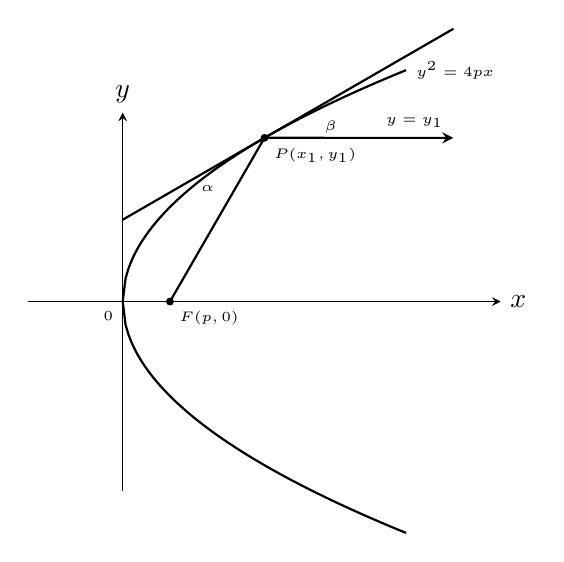
\begin{tikzpicture}[scale=1.2]
    \draw[-stealth] (-1,0) -- (4,0) node[right] {$x$};
    \draw[-stealth] (0,-2) -- (0,2) node[above] {$y$};
    \draw[thick, domain=0:3, samples=100] plot (\x, {sqrt(2*\x)}) node[right] {\tiny $y^2 = 4px$};
    \draw[thick, domain=0:3, samples=100] plot (\x, {-sqrt(2*\x)});
    
    \coordinate (F) at (0.5, 0);
    \coordinate (P) at (1.5, {sqrt(3)});
    
    \filldraw (F) circle (1pt) node[below right] {\tiny $F(p, 0)$};
    \filldraw (P) circle (1pt) node[below right] {\tiny $P(x_1, y_1)$};
    
    \draw[thick] (F) -- (P);
    \draw[thick, -stealth] (P) -- (3.5, {sqrt(3)}) node[above left] {\tiny $y = y_1$};
    
    % Recta tangente en P
    \draw[thick] (0, {1.5/sqrt(3)}) -- (3.5, {5/sqrt(3)});
    
    % Ángulos
    \node at (0.9, 1.2) {\tiny $\alpha$};
    \node at (2.2, 1.85) {\tiny $\beta$};
    \node[below left] at (0,0) {\tiny $0$};
\end{tikzpicture}
\end{center}
